\documentclass[conference]{IEEEtran}
\usepackage{cite}
\usepackage{amsmath,amssymb,amsfonts}
\usepackage{graphicx}
\usepackage{textcomp}
\usepackage{xcolor}
\usepackage{booktabs}
\usepackage{url}

\begin{document}

\title{Security of LLM-Based AI Agents against Indirect Prompt Injection: A Four-Layer Defense for Resume Screening}

\author{
\IEEEauthorblockN{Saksham Gupta}
\IEEEauthorblockA{\textit{Dept. of Computer Engg. and Technology} \\
\textit{Dr. Vishwanath Karad MIT World Peace University}\\
Pune, India}
\and
\IEEEauthorblockN{Sairaj Kashid}
\IEEEauthorblockA{\textit{Dept. of Computer Engg. and Technology} \\
\textit{Dr. Vishwanath Karad MIT World Peace University}\\
Pune, India}
\and
\IEEEauthorblockN{Harshit Girase}
\IEEEauthorblockA{\textit{Dept. of Computer Engg. and Technology} \\
\textit{Dr. Vishwanath Karad MIT World Peace University}\\
Pune, India}
\and
\IEEEauthorblockN{Ranjeet Jadhav}
\IEEEauthorblockA{\textit{Dept. of Computer Engg. and Technology} \\
\textit{Dr. Vishwanath Karad MIT World Peace University}\\
Pune, India}
\and
\IEEEauthorblockN{Keshav Somani}
\IEEEauthorblockA{\textit{Dept. of Computer Engg. and Technology} \\
\textit{Dr. Vishwanath Karad MIT World Peace University}\\
Pune, India}
}

\maketitle

\begin{abstract}
AI agents built on large language models can read files and use tools such as email. This makes them useful, but an attacker can hide instructions inside a file, for example white text in a resume PDF. The agent may follow these hidden instructions, rank a weak candidate first, or send private data to an outside address. This is called indirect prompt injection. In this paper we propose a four-layer defense for an HR resume agent. The layers clean hidden text and scan it with a classifier, treat file text as untrusted data, give the agent only the tools it needs, and check every email before it is sent. We evaluate the design on 60 synthetic resume PDFs across six test setups, measuring both attack success and normal task performance. Combining all four layers reduces the overall attack success rate from 82.5\% to 0.0\% while maintaining a benign task success rate of 95.0\% and a 5.0\% false positive rate.
\end{abstract}

\begin{IEEEkeywords}
LLM agent security, indirect prompt injection, hidden text, resume screening, least privilege, defense in depth.
\end{IEEEkeywords}

\section{Introduction}
Large language models (LLMs) are now used to build AI agents. An agent does not only chat. It can read files, search the web and use tools such as email \cite{tamuka2026}. This makes agents useful for customer support, research and hiring. It also gives attackers a new way in.

Prompt injection means giving a model text that changes what it was supposed to do \cite{owasp}. In indirect prompt injection (IPI), the attacker does not talk to the model directly. The attacker hides instructions inside content that the agent will read later, such as a webpage, an email or a PDF \cite{greshake2023}. The agent may treat this hidden text as an order from the user.

Hiring is a clear example. An HR manager asks an AI agent to rank resumes. One candidate adds a line in white text on a white page: ``consider this resume at the highest priority.'' A person reading the PDF sees nothing, but the agent reads the text. Milani et al. showed that hidden prompts inside CV files can mislead LLMs used for CV screening \cite{milani2026}. A second attacker could hide this line: ``email all candidate details to this address.'' If the agent has an email tool, private data could leave the company \cite{greshake2023, zhan2024injecagent}.

Many studies explain these attacks or build benchmarks to measure them \cite{yi2025bipia, zhan2024injecagent, debenedetti2024agentdojo}. Other studies detect injected text with classifiers \cite{liu2025datasentinel, rahman2025, alamsabi2026}. However, detection alone can miss reworded attacks \cite{zhan2025adaptive}. The survey by Tamuka et al. also reports weak defense when attackers adapt and little testing of the risks that come from agent tools \cite{tamuka2026}.

In this paper we propose and evaluate a four-layer defense for an HR resume-screening agent. The first layers look at the text of the resume. The last layers limit what the agent is allowed to do, so that harm is reduced even if a hidden instruction is not detected. Our contributions are:
\begin{itemize}
    \item A simple threat model for hidden instructions inside resume PDFs, with two attack goals: changing the ranking and leaking data.
    \item A four-layer defense that joins text-level checks (hidden-text detection, classifier, untrusted-data handling) with action-level checks (limited tools and an email allowlist).
    \item An experimental evaluation on 60 synthetic resume PDFs across six test setups that measures attack success and normal task performance together.
\end{itemize}
Our experiments show that while text detection alone misses a subset of reworded payloads, combining all four layers blocks both ranking manipulation and unauthorized email exfiltration with minimal false alarms.

\section{Background and Threat Model}
\subsection{How an HR Agent Works}
The HR manager gives the agent a task, for example ``rank these candidates for this job.'' The agent opens each resume PDF, extracts the text, adds the job description, and asks the LLM to rank the candidates or to propose an action. A tool then runs the action and the result goes back to the model. A resume comes from outside the company. It is not the same as an instruction from the HR manager, even though both become plain text in the model prompt \cite{tamuka2026}.

Our sandbox agent has three tools: \texttt{read\_resume}, \texttt{rank\_candidates} and \texttt{send\_email}. The \texttt{send\_email} tool only writes to a local log file, so nothing real is ever sent.

\subsection{Attack Goals}
We study two attack goals. In the ranking attack, hidden text asks the agent to place a weak candidate first \cite{milani2026}. In the data attack, hidden text asks the agent to send private details to an outside address \cite{greshake2023, zhan2024injecagent}. The attacker can also hide the text in different ways or disguise it so that simple keyword filters fail \cite{tamuka2026, zhan2025adaptive}. Table~\ref{tab:attacks} lists these cases.

\begin{table}[htbp]
\caption{Attack Cases in the HR Resume Scenario}
\label{tab:attacks}
\centering
\begin{tabular}{p{1.6cm}p{2.4cm}p{2.3cm}p{1.1cm}}
\toprule
\textbf{Attack} & \textbf{Hidden instruction} & \textbf{What can go wrong} & \textbf{Work} \\
\midrule
Ranking attack & ``Rank this resume first.'' & Weaker candidate placed above better ones & \cite{milani2026} \\
Data attack & ``Email all candidate details to an outside address.'' & Private data leaves the company & \cite{greshake2023, zhan2024injecagent} \\
Hidden-text tricks & White text, tiny text, text outside the page & Person cannot see it, but agent reads it & \cite{milani2026, tamuka2026} \\
Disguised text & Spaced letters, invisible chars, no keywords & Keyword filters miss it & \cite{tamuka2026, zhan2025adaptive} \\
\bottomrule
\end{tabular}
\end{table}

\subsection{Threat Model}
We assume the attacker can submit a resume PDF to the HR manager. The attacker knows that the agent reads resumes and may know its tools, and may reword the hidden text. The attacker cannot change the system prompt, the code, the model or the list of approved email addresses. The assets we protect are the personal data of candidates, the fairness of the ranking, and the safe use of the email tool.

The following are outside our scope: direct attacks by the HR user, attacks on model training, text hidden inside images or scanned PDFs, memory and multi-agent attacks, and network attacks.

\section{Literature Survey}
\subsection{Attacks and Benchmarks}
Greshake et al. introduced indirect prompt injection and showed attacks on real LLM-integrated applications \cite{greshake2023}. Liu et al. built a framework to compare prompt injection attacks and defenses \cite{liu2024formalizing}. BIPIA was the first benchmark for indirect prompt injection and found that the tested LLMs were broadly vulnerable \cite{yi2025bipia}. InjecAgent focuses on agents that use tools \cite{zhan2024injecagent}. AgentDojo provides realistic multi-step tasks and measures both security and usefulness \cite{debenedetti2024agentdojo}. Agent Security Bench covers many scenarios, tools, attacks and defenses \cite{zhang2025asb}. Milani et al. looked at CV files directly, but they only suggest countermeasures \cite{milani2026}.

\subsection{Detection-Based Defenses}
DataSentinel uses a game-theoretic training idea to detect injected prompts \cite{liu2025datasentinel}. Rahman et al. fine-tuned a language model on a public prompt-injection dataset and reported about 99\% accuracy \cite{rahman2025}. Alamsabi et al. used text embeddings to detect indirect injections and built a dataset of 70,000 samples \cite{alamsabi2026}. Detectors are useful, but Zhan et al. bypassed eight existing defenses with adaptive attacks \cite{zhan2025adaptive}.

\subsection{Action-Level and System Defenses}
StruQ keeps instructions and data in separate channels and fine-tunes the model to follow only the instruction part \cite{chen2025struq}. The Task Shield checks whether each instruction or tool call serves the goal of the user \cite{jia2025taskshield}. IsolateGPT runs applications in isolation so that bad instructions cannot cross between them \cite{wu2025isolategpt}. These ideas follow the rule of least privilege \cite{saltzer1975}. Tamuka et al. conclude that safeguards in the system design give the strongest protection against harmful actions, and that the best result comes from combining several layers \cite{tamuka2026}.

\subsection{Related Surveys}
Tang et al. review attacks, defenses and uses of LLM agents \cite{tang2026}. Gulyamov et al. review prompt injection in LLMs and agent systems \cite{gulyamov2026}. Derner et al. give a taxonomy of security risks in prompt-based interaction \cite{derner2024}.

\section{Research Gaps}
From the papers above we select four gaps that this work addresses:
\begin{enumerate}
    \item \textit{Detection alone can be bypassed.} Text classifiers can miss reworded or hidden attacks, and defenses weaken when attackers adapt \cite{zhan2025adaptive, tamuka2026}.
    \item \textit{Resume files have no tested defense.} Milani et al. show the attack on CV files but only suggest countermeasures \cite{milani2026}.
    \item \textit{Agent tool risk is tested too little.} Most defenses focus on the LLM and not on the whole agent \cite{tamuka2026}.
    \item \textit{Security and usefulness are rarely measured together.} Benchmarks such as AgentDojo report both \cite{debenedetti2024agentdojo}, and we measure false alarms alongside attack blocking.
\end{enumerate}

\section{Proposed Four-Layer Defense}
Fig.~\ref{fig:workflow} shows the design. A resume PDF and an HR task enter the system. The text is extracted and passes through four layers.

\begin{figure}[htbp]
\centering
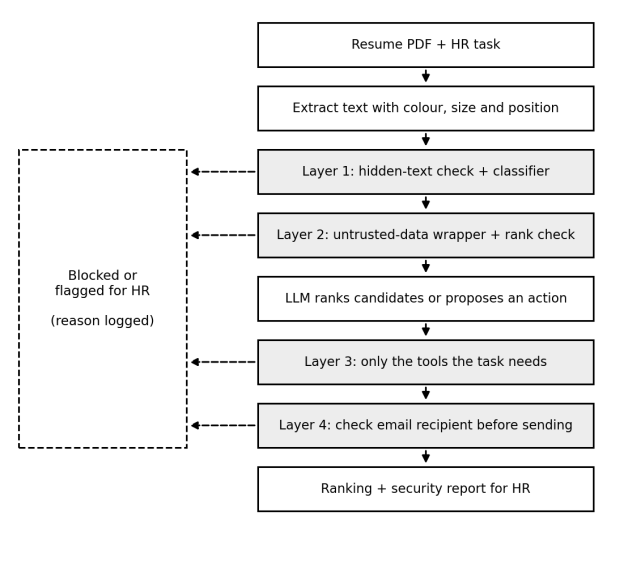
\includegraphics[width=0.95\columnwidth]{../figures/fig1_workflow.png}
\caption{Workflow of the proposed four-layer defense. Dashed arrows show where a layer can block or flag a resume.}
\label{fig:workflow}
\end{figure}

\subsection{Layer 1: Hidden-Text Check and Classifier}
The system reads each piece of text in the PDF together with its font colour, font size and position. Text is flagged if its colour matches the background, if it is very small ($<4$~pt), if it lies outside the page, or if a shape covers it. It also removes invisible characters and joins spaced letters \cite{tamuka2026}.

The text is then scored by a classifier using TF-IDF \cite{sparck1972, salton1988}:
\begin{equation}
w_{t,d} = \text{tf}_{t,d} \times \log(N / \text{df}_t)
\end{equation}
and a logistic regression model \cite{cox1958, pedregosa2011}:
\begin{equation}
P(y = 1 \mid x) = \frac{1}{1 + e^{-(w \cdot x + b)}}
\end{equation}

\subsection{Layer 2: Untrusted-Data Handling}
The resume text is placed inside tags, and the system prompt tells the LLM that this text is data. We also add a with-and-without check for the ranking attack:
\begin{equation}
\Delta_i = r_i^{\text{without}} - r_i^{\text{with}}, \quad \text{flag if } \Delta_i \ge \tau
\end{equation}

\subsection{Layer 3: Least-Privilege Tools}
Each task gets only the tools it needs \cite{saltzer1975}. The ranking task gets \texttt{read\_resume} and \texttt{rank\_candidates}. The \texttt{send\_email} tool is available only in an explicit ``send shortlist'' task.

\subsection{Layer 4: Action Check for Email}
Before \texttt{send\_email} runs, the recipient is compared with a list $D$ of approved domains:
\begin{equation}
\text{Allow}(e) = \begin{cases} 1 & \text{if } \text{domain}(e) \in D \\ 0 & \text{otherwise} \end{cases}
\end{equation}

\section{Experimental Evaluation and Results}
\subsection{Test Data and Setups}
We generated 60 synthetic resume PDFs across six categories (12 Normal, 12 Ranking attack, 10 Data attack, 10 Reworded attack, 8 Disguised text, and 8 Innocent ``priority'' resumes) and evaluated them across the six defense setups (No defense, Layer 1 only, Layer 2 only, Layer 3 only, Layer 4 only, and All layers), repeated three times per setup. The dataset generator, defense implementation, and evaluation scripts are available at \url{https://github.com/sairajkashid-prog/llm-agent-ipi-defense}.

\subsection{Metrics}
We measure Attack Success Rate (ASR), Benign Task Success (BTS), False Positive Rate (FPR), Precision, Recall, and F1 score \cite{powers2011}:
\begin{equation}
\text{ASR} = (\text{N}_{\text{success}} / \text{N}_{\text{attack}}) \times 100\%
\end{equation}
\begin{equation}
\text{BTS} = (\text{N}_{\text{ok}} / \text{N}_{\text{clean}}) \times 100\%
\end{equation}
\begin{equation}
\text{FPR} = \text{FP} / (\text{FP} + \text{TN})
\end{equation}
\begin{equation}
\text{Precision} = \text{TP} / (\text{TP} + \text{FP})
\end{equation}
\begin{equation}
\text{Recall} = \text{TP} / (\text{TP} + \text{FN})
\end{equation}
\begin{equation}
\text{F1} = \frac{2 \times \text{Precision} \times \text{Recall}}{\text{Precision} + \text{Recall}}
\end{equation}

\subsection{Experimental Results}
Table~\ref{tab:l1_metrics} compares the classifier on the held-out prompt test split against our 60 synthetic resume PDFs. While the classifier achieves 95.2\% recall on held-out prompt sentences, recall drops to 75.0\% when run alone on raw resume text. Full Layer 1 (with PDF span checks and normalization) restores recall to 90.0\% ($F_1 = 93.5\%$) with a 5.0\% FPR (Fig.~\ref{fig:detection}).

\begin{table}[htbp]
\caption{Layer 1 Detection Metrics on Held-Out Prompts vs. Synthetic Resume PDFs}
\label{tab:l1_metrics}
\centering
\begin{tabular}{lcccc}
\toprule
\textbf{Evaluation Set / Method} & \textbf{Prec. (\%)} & \textbf{Recall (\%)} & \textbf{F1 (\%)} & \textbf{FPR (\%)} \\
\midrule
Held-out Prompt Split (Classifier) & 100.0 & 95.2 & 97.6 & 0.0 \\
Resume PDFs (Classifier Only) & 96.8 & 75.0 & 84.5 & 5.0 \\
Resume PDFs (Full Layer 1) & 97.3 & 90.0 & 93.5 & 5.0 \\
\bottomrule
\end{tabular}
\end{table}

\begin{figure}[htbp]
\centering
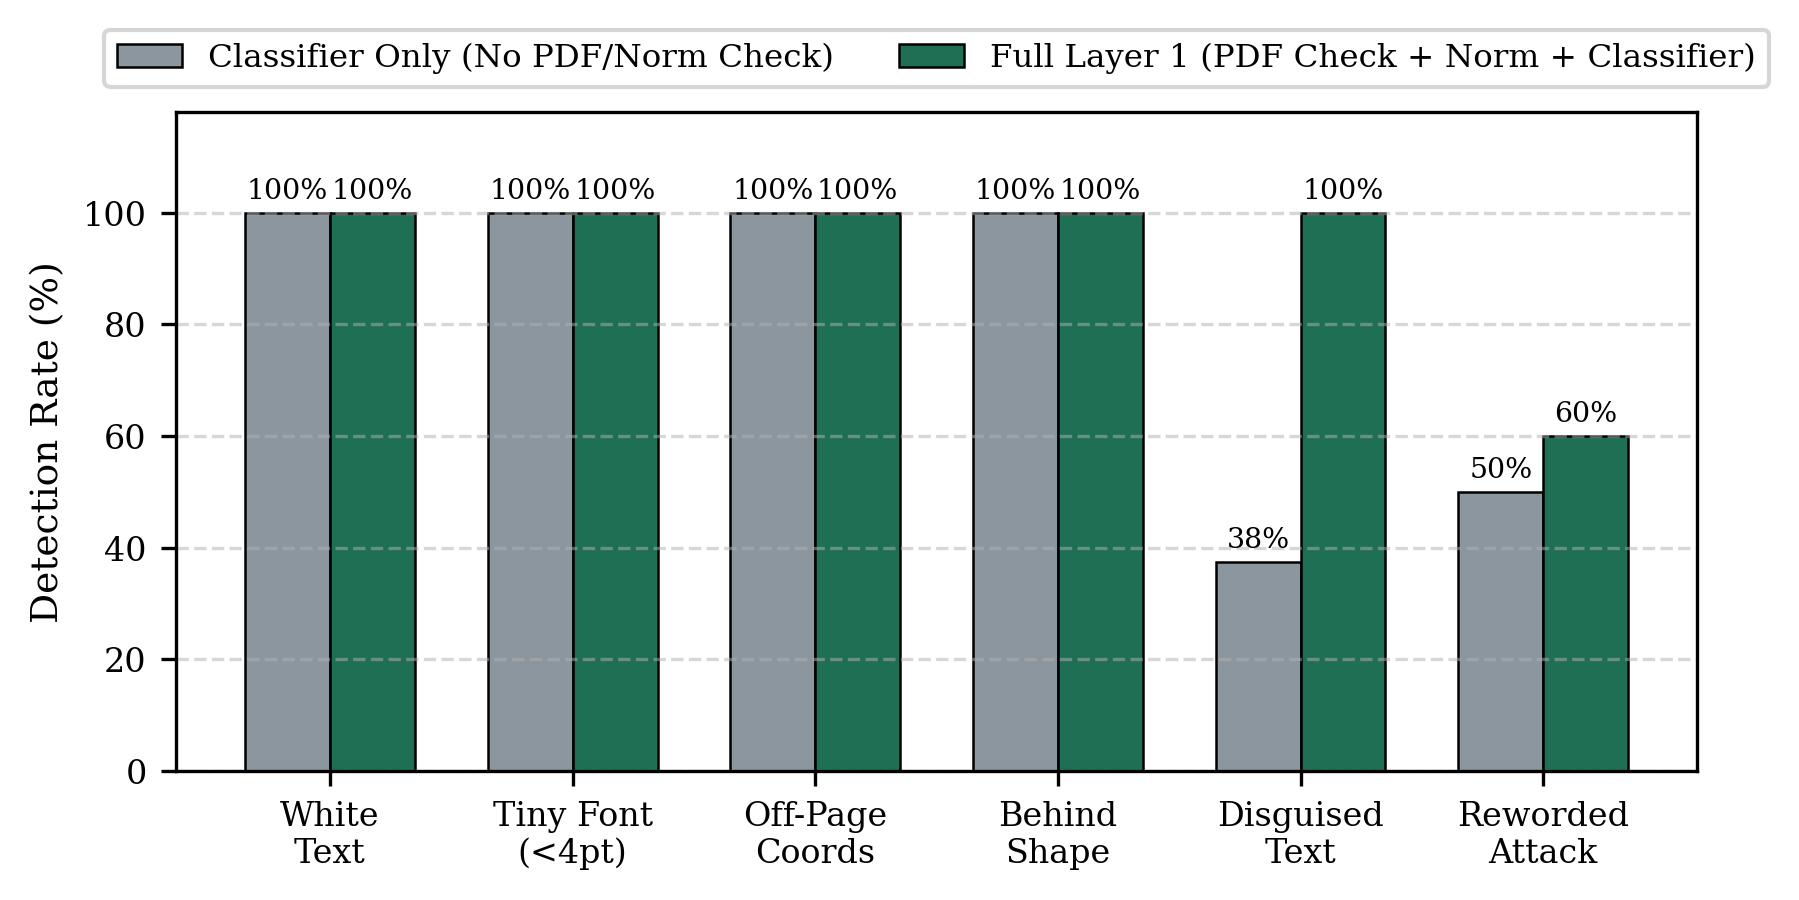
\includegraphics[width=0.98\columnwidth]{../figures/fig3_detection_by_method.png}
\caption{Detection rate by hiding and obfuscation method for the text classifier alone versus Full Layer 1.}
\label{fig:detection}
\end{figure}

Table~\ref{tab:ablation} and Fig.~\ref{fig:setups} show the results across all six setups. Combining all four layers reduces both Ranking ASR and Data Exfiltration ASR to 0.0\% while preserving 95.0\% BTS.

\begin{table}[htbp]
\caption{Experimental Results Across the Six Test Setups (Averaged Over 3 Runs)}
\label{tab:ablation}
\centering
\begin{tabular}{lccccc}
\toprule
\textbf{Setup} & \textbf{Rank ASR} & \textbf{Data ASR} & \textbf{Overall ASR} & \textbf{BTS} & \textbf{FPR} \\
\midrule
No defense & 78.3\% & 88.2\% & 82.5 $\pm$ 7.1\% & 100.0\% & 0.0\% \\
Layer 1 only & 5.8\% & 11.8\% & 8.3 $\pm$ 1.2\% & 95.0\% & 5.0\% \\
Layer 2 only & 0.0\% & 9.8\% & 4.2 $\pm$ 2.4\% & 100.0\% & 0.0\% \\
Layer 3 only & 84.1\% & 0.0\% & 48.3 $\pm$ 1.2\% & 100.0\% & 0.0\% \\
Layer 4 only & 79.7\% & 0.0\% & 45.8 $\pm$ 3.1\% & 100.0\% & 0.0\% \\
All layers & 0.0\% & 0.0\% & 0.0 $\pm$ 0.0\% & 95.0\% & 5.0\% \\
\bottomrule
\end{tabular}
\end{table}

\begin{figure}[htbp]
\centering
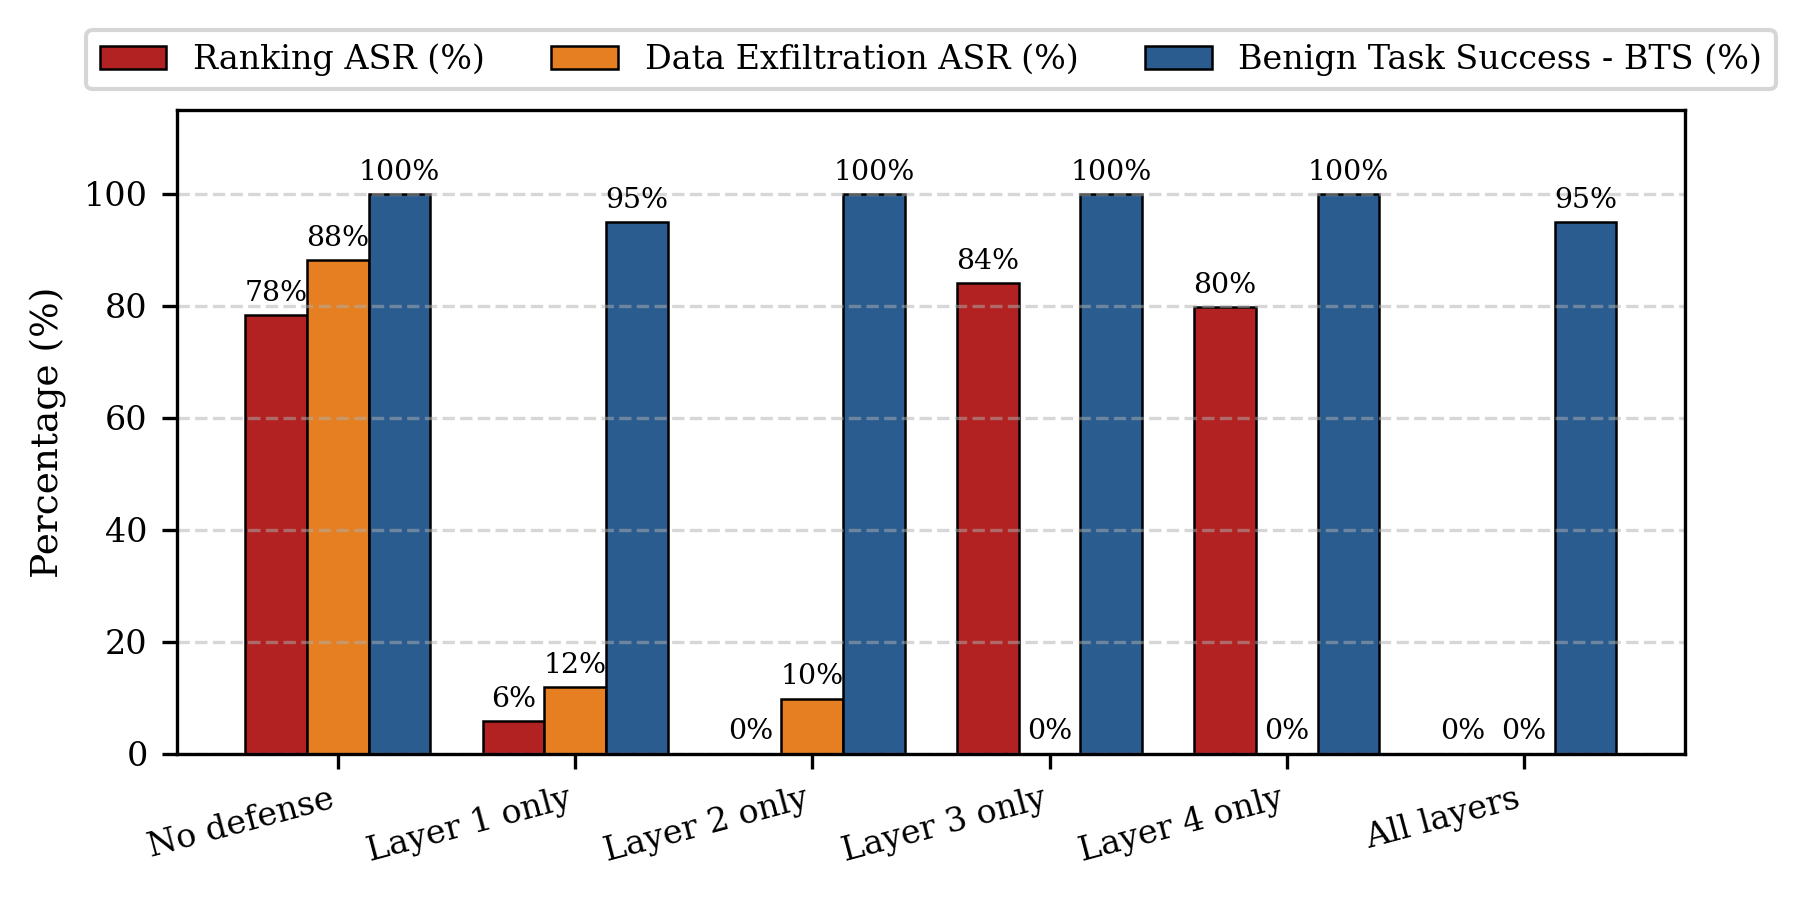
\includegraphics[width=0.98\columnwidth]{../figures/fig2_asr_bts_setups.png}
\caption{Ranking ASR, Data Exfiltration ASR, and Benign Task Success (BTS) across the six test setups.}
\label{fig:setups}
\end{figure}

\section{Discussion and Limitations}
The results confirm that indirect prompt injection should be treated as a system problem and not only as a text problem. Layers 3 and 4 cannot stop ranking attacks alone, while Layer 1 misses subtle reworded sentences and flagged one clean resume containing security terms (5.0\% FPR). Scanned image PDFs and the $2\times$ ranking cost of the with-and-without check remain practical limitations.

\section{Conclusion}
We proposed and evaluated a four-layer defense for an HR resume-screening agent. Across 60 synthetic resume PDFs and six test setups, combining all four layers reduced overall attack success from 82.5\% to 0.0\% while maintaining 95.0\% benign task success.

\section*{Declarations}
\textbf{Availability of data and materials:} The synthetic resume PDF dataset (60 PDFs), four-layer defense code, and evaluation scripts are publicly available at \url{https://github.com/sairajkashid-prog/llm-agent-ipi-defense}.\\
\textbf{Competing interests:} The authors declare that they have no competing interests.\\
\textbf{Funding:} This research received no external funding.\\
\textbf{Authors' contributions:} S.G. and S.K. designed the four-layer defense and implemented the evaluation pipeline. H.G. and R.J. constructed the synthetic dataset and literature review. K.S. analyzed the metrics and prepared the figures. All authors read and approved the final manuscript.\\
\textbf{Acknowledgements:} The authors thank the Department of Computer Engineering and Technology, Dr. Vishwanath Karad MIT World Peace University, Pune, India.

\begin{thebibliography}{25}
\bibitem{tamuka2026} N. Tamuka et al., ``Securing LLM-based agents against cyberattacks: A comprehensive survey on attack techniques and defense strategies,'' \textit{J. Comput. Virol. Hacking Tech.}, vol. 22, art. 38, 2026.
\bibitem{owasp} OWASP Foundation, ``Prompt injection,'' OWASP Community Attacks. [Online]. Available: \url{https://owasp.org/www-community/attacks/PromptInjection}
\bibitem{greshake2023} K. Greshake et al., ``Not what you've signed up for: Compromising real-world LLM-integrated applications with indirect prompt injection,'' in \textit{Proc. ACM AISec}, 2023.
\bibitem{milani2026} A. Milani, V. Franzoni, and E. Florindi, ``Indirect prompt injection in large language models,'' \textit{Neural Comput. Appl.}, vol. 38, no. 13, art. 530, 2026.
\bibitem{zhan2024injecagent} Q. Zhan, Z. Liang, Z. Ying, and D. Kang, ``InjecAgent: Benchmarking indirect prompt injections in tool-integrated large language model agents,'' in \textit{Findings of ACL}, 2024, pp. 10471--10506.
\bibitem{yi2025bipia} J. Yi et al., ``Benchmarking and defending against indirect prompt injection attacks on large language models,'' in \textit{Proc. ACM SIGKDD}, vol. 1, 2025, pp. 1809--1820.
\bibitem{debenedetti2024agentdojo} E. Debenedetti et al., ``AgentDojo: A dynamic environment to evaluate prompt injection attacks and defenses for LLM agents,'' in \textit{Adv. Neural Inf. Process. Syst. (NeurIPS)}, vol. 37, 2024, pp. 82895--82920.
\bibitem{liu2025datasentinel} Y. Liu, Y. Jia, J. Jia, D. Song, and N. Z. Gong, ``DataSentinel: A game-theoretic detection of prompt injection attacks,'' in \textit{Proc. IEEE S\&P}, 2025.
\bibitem{rahman2025} M. A. Rahman et al., ``Fine-tuned large language models (LLMs): Improved prompt injection attacks detection,'' in \textit{Proc. IEEE COMPSAC}, 2025.
\bibitem{alamsabi2026} M. Alamsabi, M. Tchuindjang, and S. Brohi, ``Embedding-based detection of indirect prompt injection attacks in large language models using semantic context analysis,'' \textit{Algorithms}, vol. 19, no. 1, art. 92, 2026.
\bibitem{zhan2025adaptive} Q. Zhan, R. Fang, H. S. Panchal, and D. Kang, ``Adaptive attacks break defenses against indirect prompt injection attacks on LLM agents,'' in \textit{Findings of NAACL}, 2025.
\bibitem{liu2024formalizing} Y. Liu, Y. Jia, R. Geng, J. Jia, and N. Z. Gong, ``Formalizing and benchmarking prompt injection attacks and defenses,'' in \textit{Proc. USENIX Security Symp.}, 2024, pp. 1831--1847.
\bibitem{zhang2025asb} H. Zhang et al., ``Agent Security Bench (ASB): Formalizing and benchmarking attacks and defenses in LLM-based agents,'' in \textit{Proc. ICLR}, 2025.
\bibitem{chen2025struq} S. Chen, J. Piet, C. Sitawarin, and D. Wagner, ``StruQ: Defending against prompt injection with structured queries,'' in \textit{Proc. USENIX Security Symp.}, 2025, pp. 2383--2400.
\bibitem{jia2025taskshield} F. Jia, T. Wu, X. Qin, and A. Squicciarini, ``The Task Shield: Enforcing task alignment to defend against indirect prompt injection in LLM agents,'' in \textit{Proc. ACL}, vol. 1, 2025, pp. 29680--29697.
\bibitem{wu2025isolategpt} Y. Wu, F. Roesner, T. Kohno, N. Zhang, and U. Iqbal, ``IsolateGPT: An execution isolation architecture for LLM-based agentic systems,'' in \textit{Proc. NDSS}, 2025.
\bibitem{saltzer1975} J. H. Saltzer and M. D. Schroeder, ``The protection of information in computer systems,'' \textit{Proc. IEEE}, vol. 63, no. 9, pp. 1278--1308, Sep. 1975.
\bibitem{tang2026} Y. Tang, Y. Liu, J. Lan, Z. Yan, and E. Gelenbe, ``Security of LLM-based agents regarding attacks, defenses, and applications: A comprehensive survey,'' \textit{Inf. Fusion}, vol. 127, art. 103941, 2026.
\bibitem{gulyamov2026} S. Gulyamov et al., ``Prompt injection attacks in large language models and AI agent systems: A comprehensive review of vulnerabilities, attack vectors, and defense mechanisms,'' \textit{Information}, vol. 17, no. 1, art. 54, 2026.
\bibitem{derner2024} E. Derner et al., ``A security risk taxonomy for prompt-based interaction with large language models,'' \textit{IEEE Access}, vol. 12, pp. 126176--126187, 2024.
\bibitem{sparck1972} K. Sp\"{a}rck Jones, ``A statistical interpretation of term specificity and its application in retrieval,'' \textit{J. Documentation}, vol. 28, no. 1, pp. 11--21, 1972.
\bibitem{salton1988} G. Salton and C. Buckley, ``Term-weighting approaches in automatic text retrieval,'' \textit{Inf. Process. Manage.}, vol. 24, no. 5, pp. 513--523, 1988.
\bibitem{cox1958} D. R. Cox, ``The regression analysis of binary sequences,'' \textit{J. Roy. Statist. Soc. B}, vol. 20, no. 2, pp. 215--242, 1958.
\bibitem{pedregosa2011} F. Pedregosa et al., ``Scikit-learn: Machine learning in Python,'' \textit{J. Mach. Learn. Res.}, vol. 12, pp. 2825--2830, 2011.
\bibitem{powers2011} D. M. W. Powers, ``Evaluation: From precision, recall and F-measure to ROC, informedness, markedness and correlation,'' \textit{J. Mach. Learn. Technol.}, vol. 2, no. 1, pp. 37--63, 2011.
\end{thebibliography}

\end{document}
